\documentclass[11pt,letterpaper,twoside]{article}
\usepackage[english]{babel}
\usepackage{amssymb,amsmath}
\usepackage{fancyhdr}
\usepackage{graphicx}

 \oddsidemargin  0in \evensidemargin 0in
 \topmargin   -0.25in \headheight 0.25in \headsep 0.25in
 \textwidth   6.5in \textheight 8.75in \marginparsep 0pt \marginparwidth 0pt
 \parskip 1ex  \parindent 0ex \footskip 20pt

\newfont{\bssten}{cmssbx10}
\newfont{\bssnine}{cmssbx10 scaled 900}

%%%%%%%%%%%%%%%%%%%%%%%
\newcommand{\whatizit}{Lecture 4: Experiments}
%%%%%%%%%%%%%%%%%%%%%%%


\pagestyle{fancy}  
\fancyhead{\bssnine STOR 155,  \whatizit}
\fancyhead[RE]{} \fancyhead[LO]{}
\fancyhead[LE]{\bssnine \thepage} \fancyhead[RO]{\bssnine \thepage}
\lfoot{} \cfoot{} \rfoot{}   


\newcommand{\var}{\mathrm{Var}}



\begin{document}



\thispagestyle{empty} \vspace*{-0.75in}

{\bssten STOR 155: Introduction to Data Models and Inference \hfill May 17, 2024 \\
Prof. Will Lassiter  \hfill Page 1 of \pageref{totalpag}}
\vspace{10pt}
\begin{center} {{\Large \bf \whatizit}} \end{center}

{\bf Four Principles of Experiment Design} \vspace{6pt}

\begin{enumerate}

\item {\bf Control}

\hspace{300pt} 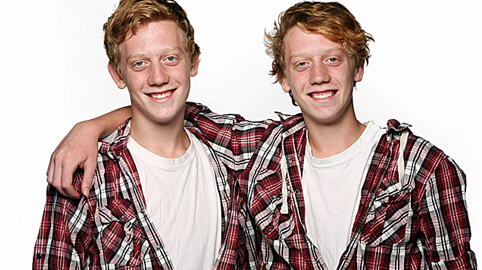
\includegraphics[scale=0.7]{images/twins.png}

\item {\bf Randomize} \vspace{80pt}

\item {\bf Replicate} \vspace{80pt}

\item {\bf Block} \vspace{80pt}

\end{enumerate}

\begin{center}
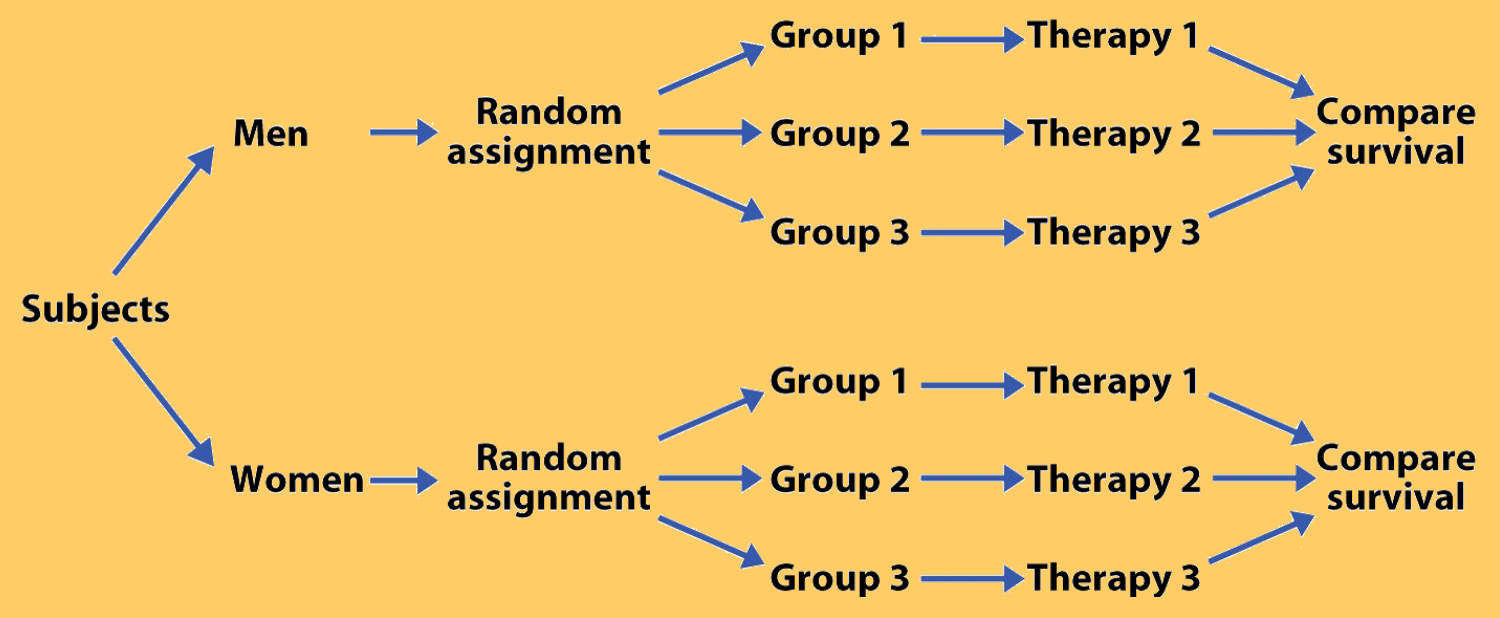
\includegraphics[scale=0.7]{images/block.png}
\end{center}

\newpage

Practice: A study is designed to test the effect of light level and noise level on exam performance of students. The researcher also believes that light and noise levels might have different effects on males and females, so wants to make sure both genders are equally represented in each group. Which of the options below is correct?

\begin{enumerate}
\item[(A)] There are 3 explanatory variables (light, noise, gender) and 1 response variable (exam performance)

\item[(B)] There are 2 explanatory variables (light and noise), 1 blocking variable (gender), and 1 response variable (exam performance)

\item[(C)] There is 1 explanatory variable (gender) and 3 response variables (light, noise, exam performance)

\item[(D)] There are 2 blocking variables (light and noise), 1 explanatory variable (gender), and 1 response variable (exam performance) \vspace{10pt}
\end{enumerate} 

{\bf More Experiment Design Terminology: Eliminating Bias}

\begin{itemize}

\item {\bf Placebo} \vspace{60pt}

\item {\bf Placebo Effect} \vspace{60pt}

\item {\bf Blinding} \vspace{60pt}

\item {\bf Double-Blind} \vspace{60pt}

\end{itemize}

\newpage

{\bf Experiments vs.\ Observational Studies: A Comparison} \vspace{6pt}

\begin{center}
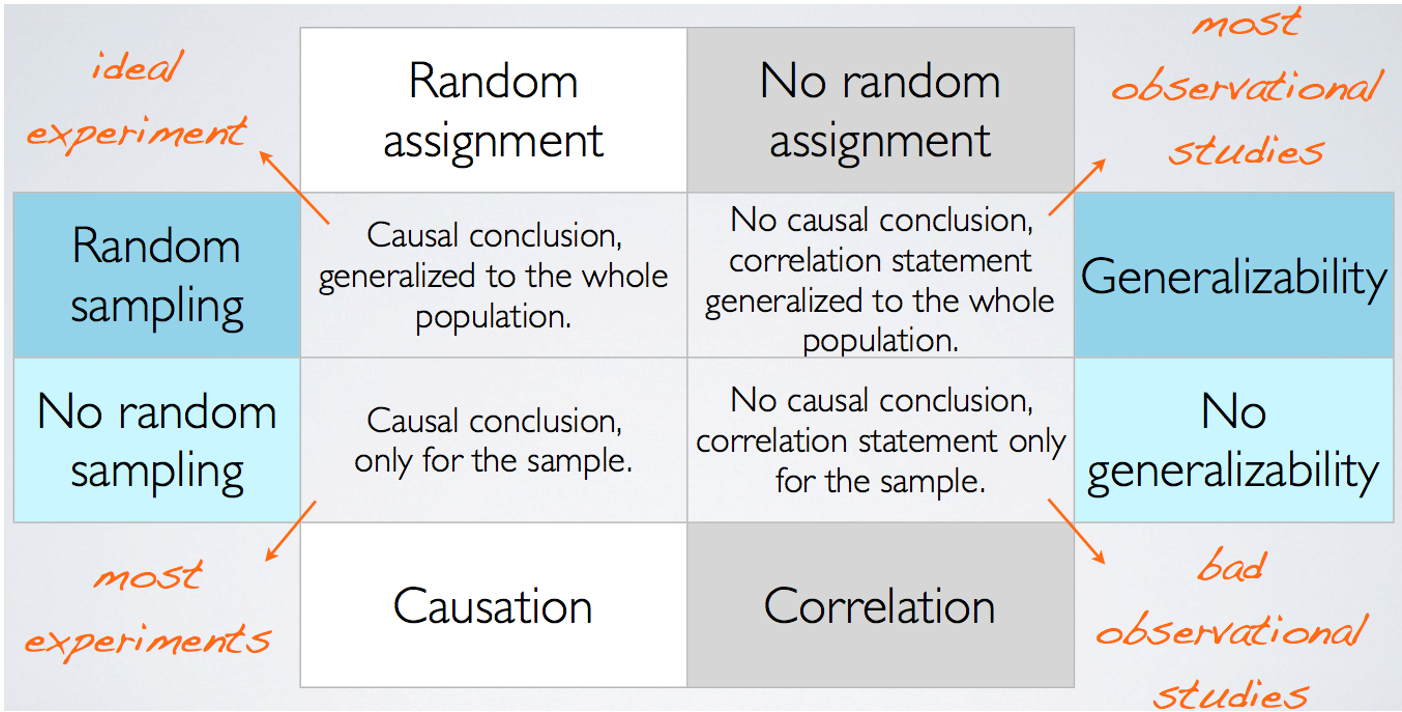
\includegraphics[scale=0.75]{images/random.png}
\end{center}

\vspace{20pt}

More practice: Choose the option(s) below that describe differences between observational studies and experiments.

\begin{enumerate}

\item[(A)] Experiments take place in a lab while observational studies do not need to.

\item[(B)] In an observational study we only look at what happened in the past.

\item[(C)] Experiments use random assignment while observational studies do not.

\item[(D)] Observational studies are completely useless since no causal inference can be made based on their findings.

\item[(E)] Experiments involve active intervention/treatment, while observational studies are passive. 

\end{enumerate}



\label{totalpag}
\end{document}